\documentclass[11pt, oneside]{article}   	% use "amsart" instead of "article" for AMSLaTeX format
\usepackage{geometry}                		% See geometry.pdf to learn the layout options. There are lots.
\geometry{letterpaper}                   		% ... or a4paper or a5paper or ... 
%\geometry{landscape}                		% Activate for rotated page geometry
%\usepackage[parfill]{parskip}    		% Activate to begin paragraphs with an empty line rather than an indent
\usepackage{graphicx}				% Use pdf, png, jpg, or eps§ with pdflatex; use eps in DVI mode
								% TeX will automatically convert eps --> pdf in pdflatex	
\usepackage{fullpage}
\usepackage[latin1]{inputenc}
\usepackage[cyr]{aeguill}
\usepackage[francais]{babel}

\usepackage{physics}
\usepackage{mathrsfs}

\usepackage{color}

\usepackage{enumitem}

\usepackage{cite}


%\renewcommand \thechapter{\Roman{chapter}}
\renewcommand \thesection{ \Roman{section}}
\renewcommand \thesubsection{ \arabic{subsection}}



\usepackage{amsmath}
\usepackage{amssymb}


\newcommand{\icol}[1]{% inline column vector
  \left(\begin{smallmatrix}#1\end{smallmatrix}\right)%
}


\title{Compte-rendu du CAT}
\author{Pierre Bataille, David Rey}
\date{}							% Activate to display a given date or no date

\begin{document}
\maketitle





\section*{Introduction}
\paragraph{}
%%Pr�sentation de la parit� avec une petite explication en passant par quelques notions de th�orie des champs.:
Since the beginning of the 20$^{th}$ century with the rise of both quantum mechanics and Einstein's theory of relativity, physicists have tried to unify the laws of physics in one model.
A milestone of particular importance is the Noether's theorem, which associated a conserved quantity to a specific symmetry. For instance: a process where energy is conserved is invariant with respect to time. 
Here is a list of the 6 symmetries that are associated to conservation laws:
\begin{itemize}[ label=\textbullet ]
\item conservation of energy is associated to the invariance with respect to time.
\item conservation of momentum is associated to the invariance by translation.
\item conservation of angular momentum is associated to the invariance by rotation.
\item conservation of parity (P) is associated to the symmetry of reflexion with respect to a point.
\item conservation of charged (C) conjugaison is associated to the change from particle to antiparticle.
\item conservation by time reversal (T) is associated to change of the time t by -t.
\end{itemize}
The three first laws are respected in all physical processes. This is not the case of the charge conjugaison, the time reversal symmetry and the parity.
At first they were seen as fundamental laws of nature, but physicists later discovered that they could be violated.
The only global symmetry that still holds is the product of the three of these quantities. This is called the CPT theorem.



%%%% D�finition de la parit�
\paragraph{}
The idea behind parity is simple: let us consider a specific experiment, or, more broadly speaking, a physical process.
This experiment is said to preserve parity if both the experiment and its mirror image yield results that are the symmetric of each other with respect to the mirror. 
In order to study parity violating processes, we will first give an overview of what the weak interaction is, as it enables parity non-conserving processes. We will then describe the experiment conducted by C.S. Wood on a cesium beam, which was the first measurement of the anapole moment, a quantity strongly associated with the weak interaction and parity non-conservation.



\section{The weak interaction: the interaction which does not conserve parity.}
\paragraph{}
The electromagnetic interaction conserves parity and there is no sign that the strong nuclear force violates the conservation of parity either.
Among the three fundamental interactions described in the standard model of particle physics, the weak interaction is thus the only one known to violate parity conservation.




\subsection{A brief presentation of the weak interaction}
\subsubsection{The $\theta-\tau$ puzzle}
%%% Description de l'interaction avec structure historique
%% Lee et Yang
During the 50's, some spectacular improvements were made in particle physics, and a lot of new particles where being discovered. While physicists were trying to classify all these new strange objects, a group stood out: the K mesons\cite{Daussy}.
K mesons are bound states of two quarks which are short lived. In this group, there are two particles, $\theta$ and $\tau$, which have very similar properties and more specifically, have the same parity.
These particles had the unusual property to decay via different processes, one which preserves parity and the other which does not.
This problem was known as $\theta-\tau$ puzzle.
This led two chinese-american physicists, T.D. Lee and C.N. Yang, to suggest that parity was not conserved in processes involving the weak interaction \cite{LeeYang}.
At the end of their article, they mentioned some experiments which could lead to the investigation of the parity violation in different physical process.  

%% Exp�rience de Wu et la premi�re exp�rience
\subsubsection{Parity violation in the $\beta$-decay of the cobalt 60}
A year after the publication of the Lee-Yang article, another chinese-american physicist called C. S. Wu shed more light on parity violating processes by studying the $\beta$-decay of the cobalt 60\cite{Wu}. 
His team was cooling a crystal containing some cobalt 60, a radioactive isotope, which decays as follow: 
\begin{equation}
Co^{60} \rightarrow Ni^{60} + e^{-} + \nu + \bar{\nu}
\end{equation}
In order to study parity violation, the cryostat was placed in a magnetic field. A detector placed at one end of the cryostat was used to detect the electron.
Assuming the parity is conserved, the spatial distribution of the direction of emission should be insensitive to the orientation of the magnetic field. 
However, the actual emission behaves very differently: the electrons are emitted preferentially in the direction opposite to the nuclear spin. 
After this discovery, Lee and Yang were rewarded by Nobel Price of physics for their prediction. 

\begin{figure}[h!]
	\centering
	\makebox[\textwidth][c]{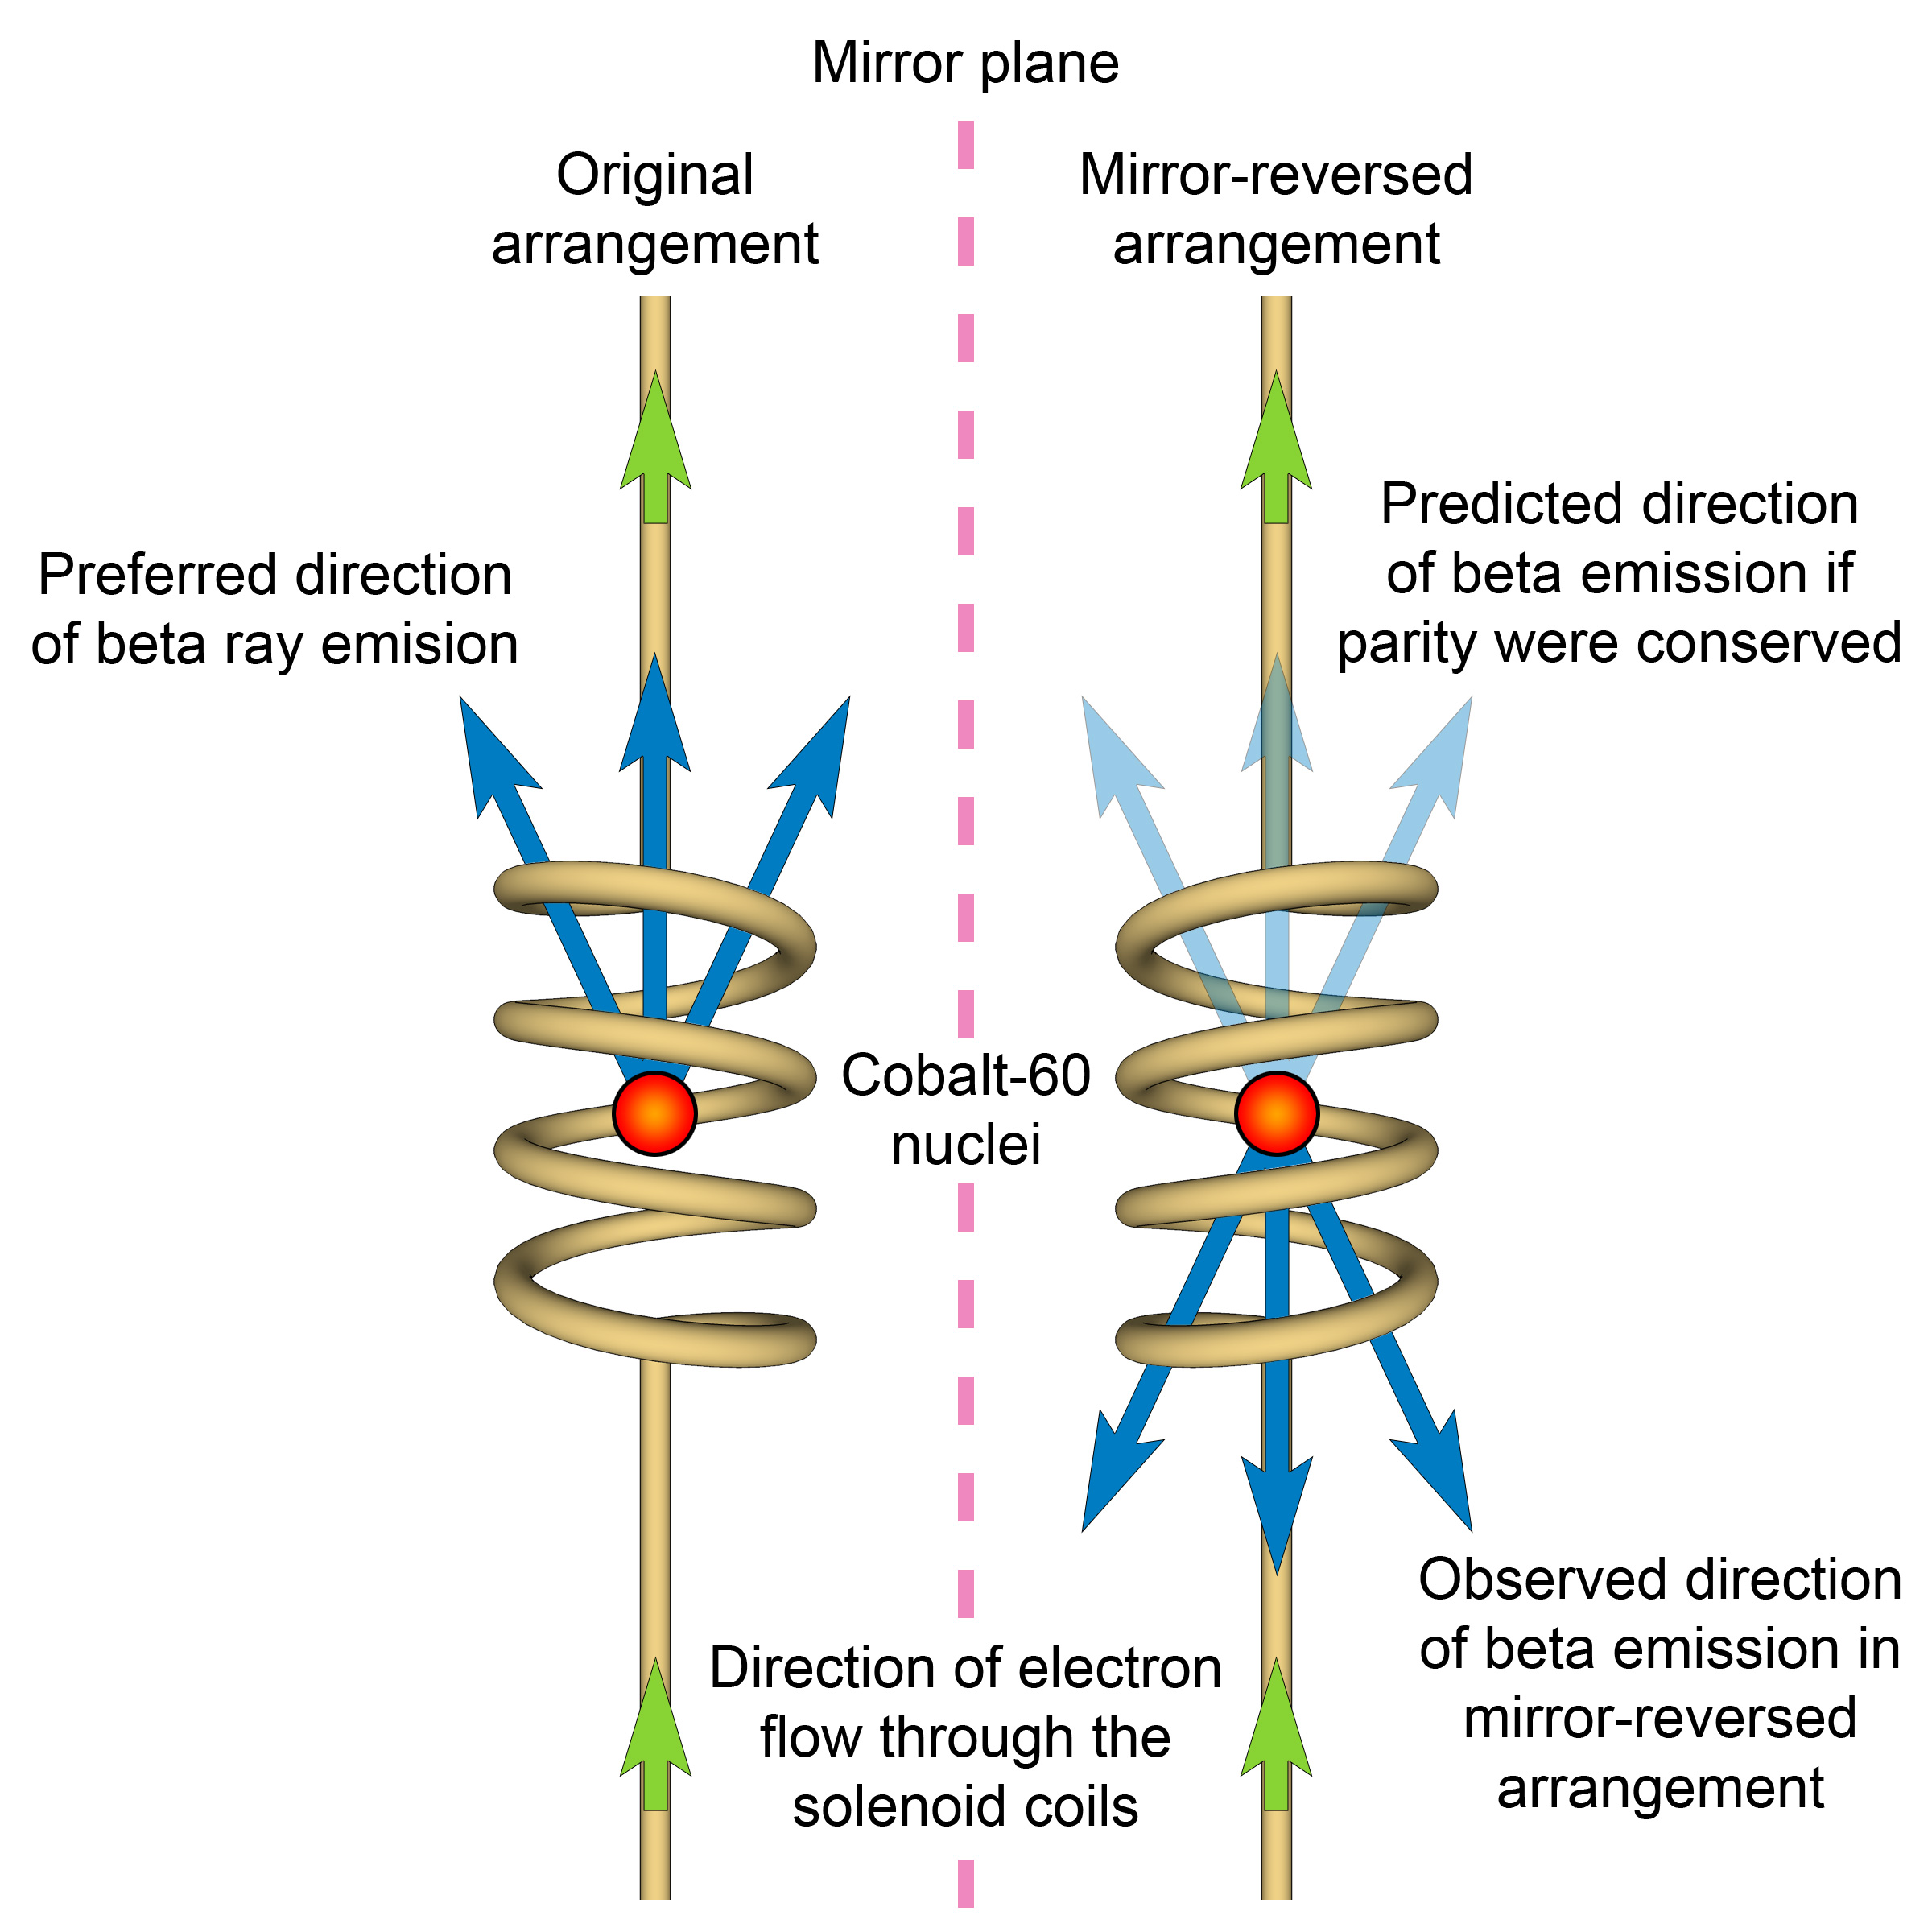
\includegraphics[width=0.35\textwidth]{wu_experiment.jpg}}
	\caption{The two configurations of the experiment are the exact symmetric of each other with respect to the mirror plane. Parity would be conserved if the $\beta$ ray direction was the same in both cases, but Wu observed that the direction of emission was reversed between the two configurations.}
	\label{fig:wu}
\end{figure}

%% Th�orie unifi�e et vague description de l'interaction faible au travers des diff�rents param�tres.
\subsubsection{Intermediate vector bosons}

Salam, Glashow and Weinberg independantly formalized the weak interaction at the end of the 60's\cite{Marrel}.
%At the end of the 60's, Salam, Glashow and Weinberg independantly formalized the weak interaction \cite{Marrel}.
%It can be seen as a generalization of the electromagnetic interaction, where the electric charge is replaced by the weak hypercharge.
%The main concept behind this theory is to consider that each spinor can be decomposed into two different contributions: 
%\begin{itemize}[ label=\textbullet ]
%\item the lefthand part: $ \psi_{L} = \frac{1-\gamma^{5}}{2} \psi $  
%\item the righthand part: $ \psi_{R} = \frac{1+\gamma^{5}}{2} \psi $
%\end{itemize}
%These two components behave differently. The lefthanded part of a fermion behaves as a doublet ($\icol{e_L\\\nu_L}$ and $\icol{u_L\\d_L}$), whereas the righthand part will behave as a singlets ($e_{R}$, $u_{R}$ and $d_{R}$).
%Neutrinos do not have a righthand part, while anti-neutrinos do not have a lefthand part.


The weak interaction can be mediated by three different bosons: $W^{+}$, $W^{-}$ and $Z^{0}$.
$W^{+}$ ($W^{-}$) has a charge of $+\textit{e}$ (resp. $- \textit{e}$), while Z$^{0}$ is a neutral particle. 

In this document, we will focus on weak interaction in atoms, and more particularly on neutral current weak interactions, which are mediated by Z$^{0}$.


\begin{figure}[h!]
\centering
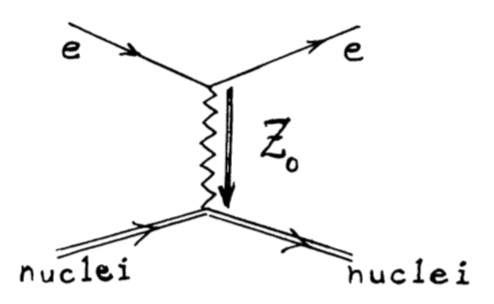
\includegraphics[ width=8cm ]{feynmandiag}
\caption{Exemple of a process involving the weak interaction that we have to consider in atomic physics.}
\end{figure}




\subsection{Measuring parity non-conservation in neutral atoms}
%% pouvoir rotatoir d'une vapeur atomique
\subsubsection{Optical activity of an atomic gas}

A possible way to measure parity non-conservation in neutral atoms is to measure their optical activity. Unlike chiral molecules, atoms are centrally symmetric. Thus, assuming that parity is conserved, they should have no optical activity. Any residual optical activity is thus the sign of processes which violate parity \cite{bouchiat}.   

%%% ins�rer image de bouchiat et al pour l'explication de la violation de la parit� + citation 


%% comment prendre en compte les diff�rents couplage e- -nuc, nuc-nuc et e- - e-
\subsubsection{The $Z^3$ law}

At its core, the weak interaction couples 2 fundamental fermions (for instance, an electron and a quark\cite{Marrel}). 
However, we can calculate the weak current between more complex fermions by adding the contribution from their fundamental constituents. 
Parity non-conservation stems from:
\begin{itemize}[ label=\textbullet ]
\item the coupling between nucleons and electrons

\item the coupling between electrons
\end{itemize}

The contribution due to the coupling of electrons is negligible in most cases.
The contribution arising from the coupling between nucleons and electrons increases roughly as $Z^3$: the heavier the element, the larger the coupling. This is important when choosing which atom to use. Cesium is a good choice : it has a high Z ($Z=55$), but its electronic structure remains simple enough to have a minimal error on calculations.
 % Pr�ciser que l'int�r�t de faire ces calculs et de les comparer � l'exp�rience, c'est de voir si il y a quelque chose que le mod�le standard ne d�crit pas (dans le cas o� les calculs et l'exp�rience ne collent pas). 
\subsubsection{The anapole moment}

\begin{figure}[h]
\centering
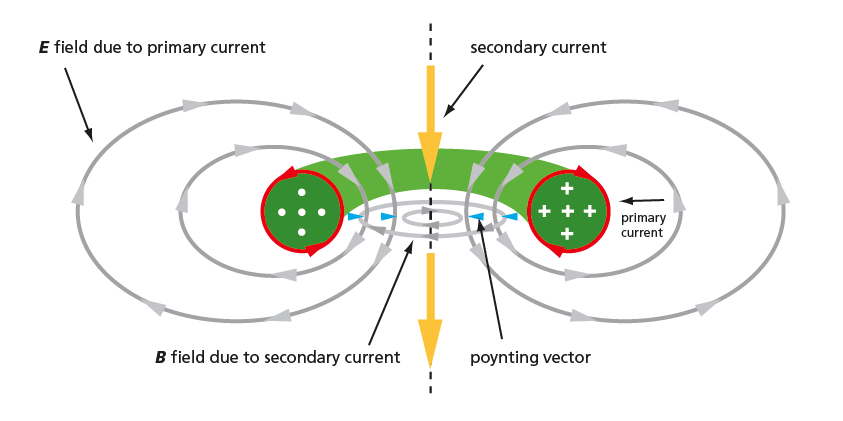
\includegraphics[ width=12cm ]{b_1_q_0_p_0.jpg}
\caption{This figure shows all the fields generated by the current around a toroid. One can see that outside the toroid there is a primary electric field. This field violates parity.}
%%% CHANGER CETTE L�GENDE
\end{figure}

The anapole moment was first described by Zel'dovich \cite{zeldovich}.
It is an electromagnetic multipole which violates the parity. %%% citation Flambaum
It can be seen as the field generated by a current passing through a self-inductive dipole on a toroid.

Simply put, the anapole moment violates parity because the processes at its core (which happen inside the nucleus) violate the conservation of parity.
These processes induce a charge displacement inside the nuclear structure, which creates a magnetic current and a spin, the anapole moment.  
This is the parity violating process which is investigated in the cesium experiment which will be described later on.

\subsection{Parity violation: what is at stake?}

\paragraph{}
Besides the fact that studying weak interaction is really challenging, there is some reason to study in depth the effect of weak interaction in the context of atomic physics. 
One of the most fascinating hypothesis concerns the homochirality of life on earth: the molecules which compose living organisms are almost exclusively left-handed. 
Parity non-conservation might be at the heart of this oddity. It is however competing with many other theories.

\paragraph{}
Another force driving the research on parity non-conservation is the standard model.
So far the standard model of particle physics is the most advanced theory ever formulated, but some parameter inside this model have to be measured. 
This is the case for constants related to the weak interaction, such as the parameter C$_{u-v}$. 
It is linked to the coupling between electrons and nucleons via the spin and should be extremely small. 
The idea behind such measurement is to test the limits of the standard model by comparing the experimental results and the theoretical results given by the standard model.


%\begin{enumerate}
%\item D�tails sur l'interaction faible avec les exp�riences historiques (Wu). On d�taillera aussi ce qui a amen� les gens � se poser la question de l'importance de la chiralit� en premier lieu (chiralit� gauche dans la nature en particulier), i.e. tout ce qui rel�ve des manifestations "macroscopiques" de la violation de la parit�. On y fera le lien avec la physique des particules.
%\item Quels sont les effets qui se manifestent en physique atomique.
%\item Pourquoi l'exp�rience sur le c�sium est vraiment int�ressante.
%\item Expliquer les enjeux li�s � la violation de la parit�.
%\end{enumerate}




\section{Measurement of parity non conservation and an anapole moment in cesium}

One possible way to observe parity non-conservation in atomic physics is to probe the transition forbidden by selection rules (which rely on parity conservation). This is what Wood et al. did in their paper "Measurement of parity non conservation and an anapole moment in cesium" \cite{AnapoleCesium}.

Probing weak interaction on forbidden transitions is a way to reduce the influence of electromagnetic interactions, which are able to generate effects that could be confused for parity non-conservation.
However, even when driving a forbidden transition, the electromagnetic interactions remain superior to the weak interactions.

The first person to successfully probe a forbidden transition was E. Commins in 1981. However, he used thallium, for which the theoretical calculations lack precision: with error bars of up to 30\% on both the experimental data and the theoretical results, it was impossible to see whether or not there was a discrepancy between the two.

Cesium, as we've said before, is better suited for this kind of test, as its electronic structure is very simple, which reduces the uncertainty on theoretical calculations.

The forbidden transition that is driven in this experiment is the 6S to 7S transition. The relevant energy levels are shown in fig \ref{fig:cs}.

\begin{figure}[h!]
	\centering
	\makebox[\textwidth][c]{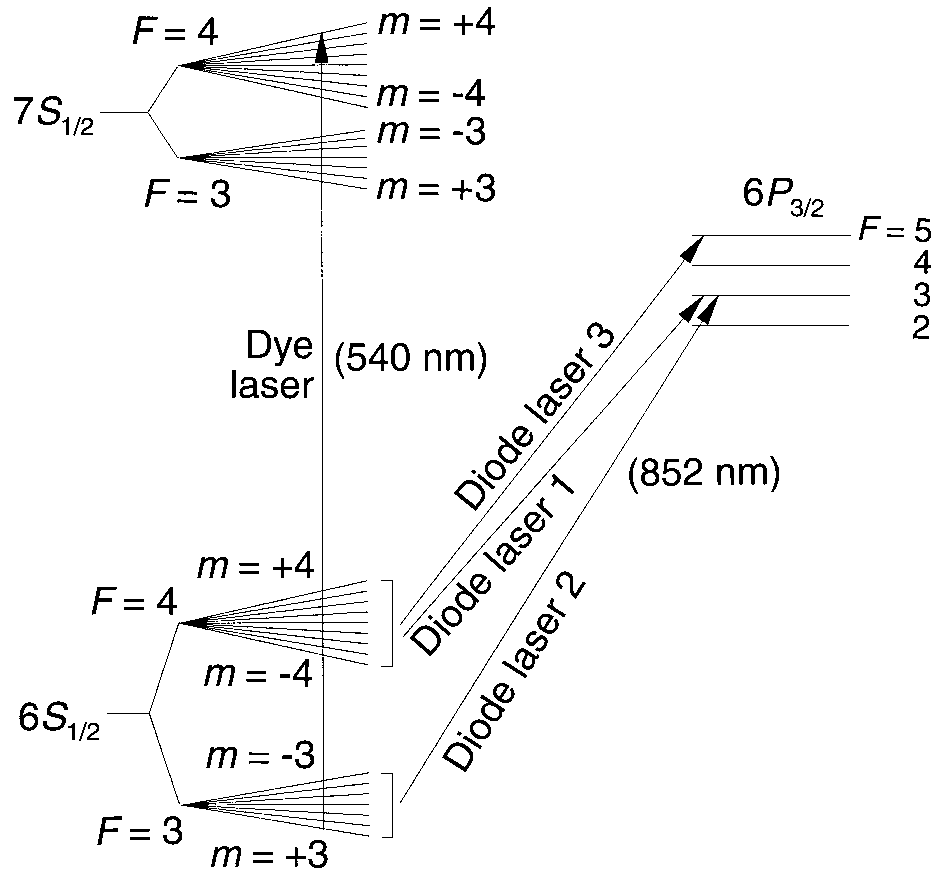
\includegraphics[width=0.5\textwidth]{cesium_states.png}}
	\caption{The energy level diagram.}
	\label{fig:cs}
\end{figure}

This transition should be forbidden by the parity selection rule (assuming there are no electric fields or weak neutral currents). However, because of the parity violating weak neutral current, which mixes a small amount of the P state into the 6S and 7S states, a small dipolar transition between 6S and 7S becomes possible. Let us write its amplitude $A_{PNC}$. A DC electric field is also applied to mix a larger amount of the P and S states, thus allowing to get a decent signal to observe the PNC transition. However, this also gives rise to a transition amplitude between 6S and 7S that we will call $A_E$, and which is typically $10^5$ times larger than $A_{PNC}$. Under certain conditions regarding the polarization of the laser beams, these two amplitudes will interfere. 

Two forbidden transitions are probed: the $6S_{F=3}$ to $7S_{F=4}$ and the $6S_{F=4}$ to $7S_{F=3}$. For both transitions, the only Zeeman states that are populated and used as a starting point for excitation are those with extreme values of the magnetic quantum number ($m=\pm 3$ and $m=\pm 4$ respectively).
The transition rate is:
\begin{equation}
	R = |A_E+A_{PNC}|^2 \approx \beta^2 E_{x}^2 \epsilon_{x}^2 C_1(F,m,F',m')+2\beta E_x \epsilon_x 2p \text{Im}(\epsilon_x) \text{Im}(E1_{PNC}) C_2(F,m,F',m')
	\label{eq:rate}
\end{equation}

where :

\begin{itemize}
	\item $\beta$ is the tensor transition polarizability
	\item $E_x$ is the DC electric field
	\item $C_1$ and $C_2$ are combinations of Clebsch-Gordan coefficients
	\item p is the handedness of the polarization
	\item Im($E1_{PNC}$) characterizes the amount of mixing between the S and P states, and is thus characteristic of the PNC weak neutral current interaction.
\end{itemize}

In both cases, the value of $\frac{A_{PNC}}{A_E}$ is measured. It is possible to distinguish $A_{PNC}$ from the others as it modulates with the reversal of E, m and p. All in all, there are five parity reversals during the experiment, all coming from different sources (reversal of the polarization of the optical pumping light, reversal of the magnetic field in the 6S-7S excitation region, etc...). This is great as it enables the elimination of potential systematic errors.

%\subsection{Apparatus} 
%A schematic of the apparatus is shown in fig. \ref{fig:exp}.

%\begin{figure}[h!]
%	\centering
%	\makebox[\textwidth][c]{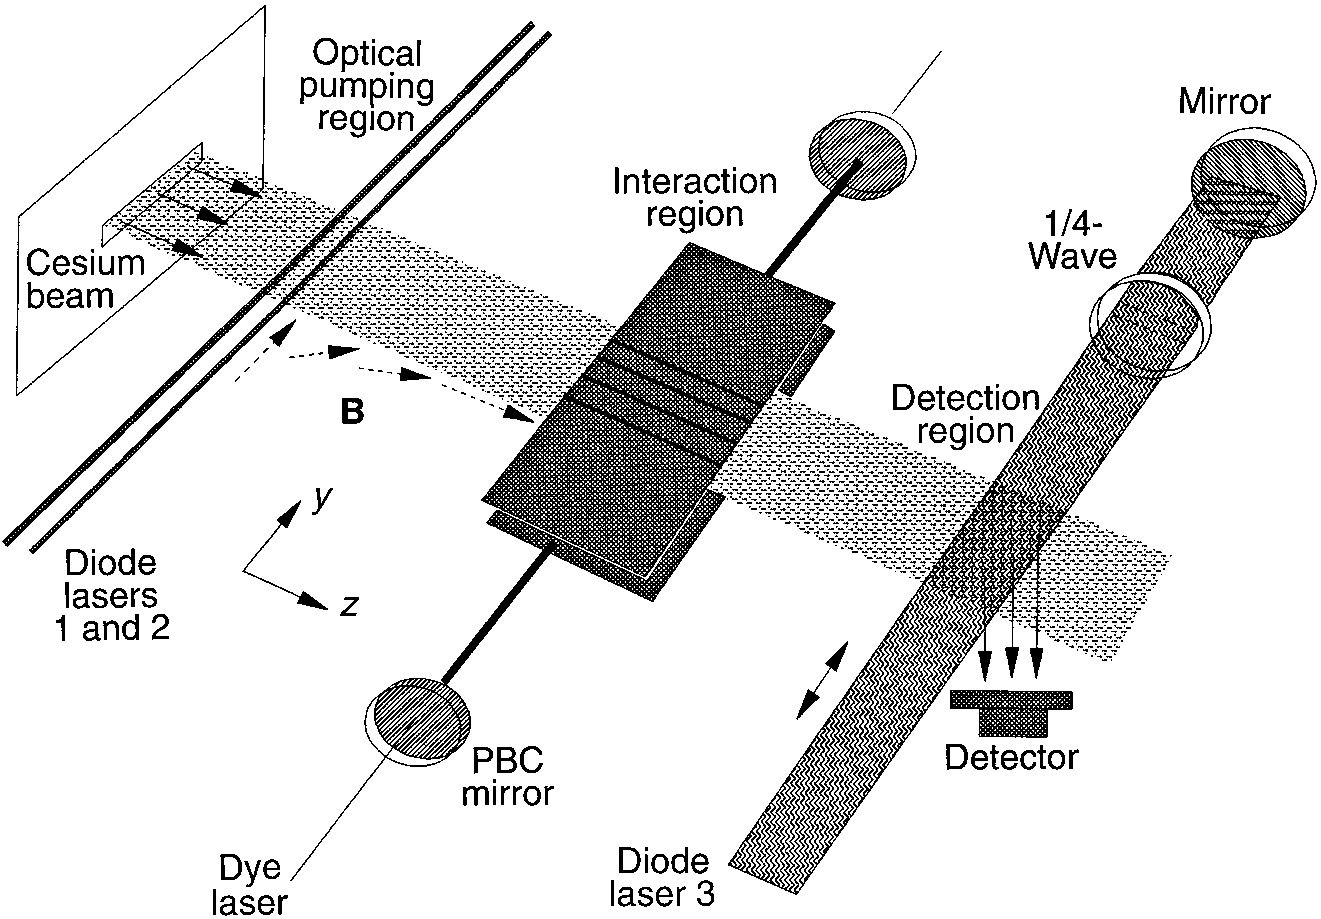
\includegraphics[width=0.5\textwidth]{cesium_exp.png}}
%%	\caption{Diagram of the experimental setup}
%	\label{fig:exp}
%\end{figure}

%An effusive beam of cesium is produced by an oven. Diode laser 1 and 2 optically pump the cesium 

\section*{Conclusion}

Parity non-conservation processes are very subtle phenomena which require high precision measurements. The development of new techniques, in particular using trapped molecules, could enable testing further and further the standard model, and better our understanding of the weak interaction.

\bibliography{bibliothese.bib}
\bibliographystyle{unsrt}


\end{document}  
